
\documentclass{article}
\usepackage{amsmath} %Never write a paper without using amsmath for its many new commands
\usepackage{amssymb} %Some extra symbols
\usepackage{makeidx} %If you want to generate an index, automatically
\usepackage{graphicx} %If you want to include postscript graphics
%%%  \usepackage{mystyle} 
%Create your own file, mystyle.sty where you put all your own \newcommand statements
%%%
%%%
\usepackage{amscd}

\usepackage{Sweave}


%%\VignetteIndexEntry{Examples of Grade Scaling from package:ProfessR}

%%% \usepackage{Sweave}

\begin{document}

%%%\renewcommand\floatpagefraction{.9}
%%%\renewcommand\topfraction{.9}
%%%\renewcommand\bottomfraction{.9}
%%%\renewcommand\textfraction{.1}
%%%\setcounter{totalnumber}{50}
%%%\setcounter{topnumber}{50}
%%%\setcounter{bottomnumber}{50}

\setkeys{Gin}{width=0.9\textwidth}



\numberwithin{equation}{section}

%%%   \SweaveOpts{prefix.string=rseis}



\author{Jonathan M. Lees\\
University of North Carolina, Chapel Hill\\
Department of Geological Sciences\\
CB \#3315, Mitchell Hall\\
Chapel Hill, NC  27599-3315\\
email: jonathan.lees@unc.edu\\
ph: (919) 962-0695
}
%%  \address{University of North Carolina, Chapel Hill}
%% \contact{Jonathan M. Lees}
%% \contactaddress{Department of Geological Sciences, CB #3315, Mitchell Hall, Chapel Hill, NC  27599-3315}
%% \contactemail{jonathan.lees@unc.edu}
%% \contactphone{(919) 962-0695}
\title{Grade Curve Analysis in R}
\date{September, 2007}

\maketitle


\begin{abstract}
This vignette is intended to instruct users on how to set up
and manipulate routines to curve (scale) a set of grades
from an exam in a large class.  The curves can be generated 
automatically, based on statistical distribution,
or interactively by graphical inspection of
a  plot of the grade distribution.

\end{abstract}


\section{Grade Curve}

Given a (possibly) large set of
grades from an exam, or a course, we need to determine 
where letter-grade cut-offs should be set for 
numerical scores.
This package provides help on 
how to scale the scores  and, finally,  assign 
letter-grades  associated with each numerical test score.

The programs in ProfessR provide a quick interactive 
procedure for quickly assigning the scaled letter-grades.
As an example,  make an artificial set of gaussian distributed grades,
\begin{Schunk}
\begin{Sinput}
> g = rnorm(n = 200, m = 82, sd = 10)
> g[g > 100] = 100
> g[g < 1] = 1
\end{Sinput}
\end{Schunk}

For now we want to establish divisions for
the grades, temporarily, and later we will show how
one can extract the divisions interactively.
Using the boxplot function we calculate the quartiles
and use these for now,
\begin{Schunk}
\begin{Sinput}
> B = boxplot(g, plot = FALSE)
> divs = c(min(g), B$stats[1:4] + diff(B$stats)/2, max(g))
\end{Sinput}
\end{Schunk}
The divisions divide the scores
into groups that are assigned grades.
The use of the boxplot function often provides good 
guides for dividing a large set of 
real test grades.
The main code in ProfessR now can plot the grades and
\begin{Schunk}
\begin{Sinput}
> library(ProfessR)
> get(getOption("device"))(width = 12, height = 7)
> D1 = do.grades(g, divs = divs, tit = "GEOL 105 Exam 1")
\end{Sinput}
\begin{Soutput}
Grade divisions:
51.32913
66.48156
79.05582
85.63842
94.48364
100
Letter Grade Distribution:
1 A+ 13
2 A 3
3 A- 10
4 B+ 14
5 B 11
6 B- 21
7 C+ 20
8 C 16
9 C- 19
10 D+ 30
11 D 20
12 D- 11
13 F 12
Numeric Grade Distribution:
1 100 13
2 96 0
3 92 0
4 88 0
5 84 0
6 80 0
7 76 0
8 72 0
9 68 0
10 64 0
11 60 0
12 56 0
13 52 0
[1] "Mean Score= 75.2345307157419"
\end{Soutput}
\end{Schunk}
display a histogram of the grades with divisions
illustrated (vertical dashed lines)  and grade  cut-offs marked.
In addition other statistics are shown, including the mean,
and standard deviations from the mean.

Normally the automatic method does not work to complete satisfaction,
so the program can be run interactively by 
removing the  divs argument.
The user must then
select the cut-offs graphically by clicking 4 times on the
plot to set  the desired distribution of grades.
This allows an instructor to shift the
cut-off points slightly depending on
the slight variations that often occur on real test scores.
For example if there is 
a small peak in near the boundary between A and B,
the instructor may wish to give a slight boost
to those students by bumping them up to an A- grade
if they autoatically would fall into the B+ category.


The out put of the do.grades routine includes all the original grades,
the scaled values and the letters associated with those 
scores.  The letters are assigned by
the divisions and linearly interpolated between
division marks to get plus and minus categories (A-, B+, etc...) .
The scaled scores are stored for later use, say for averaging 
hourly exams and the scaled final exam.
(Since the hourly exams and the final exams are scaled individually,
the final course grade , which is a weighted average of these
test scores would not necessarily be scaled).

Once the divisions are set,
a final presentation  plot can be generated by using the 
divisions extracted from the user input via the locator() 
function.  For this vignette, however,
we replace the user's input with the 
generated divisions determined above, although in 
a real situation this would not 
be used.  In this example we load a set of real data
recorded on the second exam from a geology test
at the University of North Carolina,
\begin{Schunk}
\begin{Sinput}
> data(E2grades)
> g = E2grades
> B = boxplot(g[g > 1], plot = FALSE)
> divs = c(min(g), B$stats[1:4] + diff(B$stats)/2, max(g))
> G1 = do.grades(g, divs = divs, tit = "GEOL 105 Exam 1")
> J = jist(G1$hist, G1$grades, G1$lett)
\end{Sinput}
\end{Schunk}
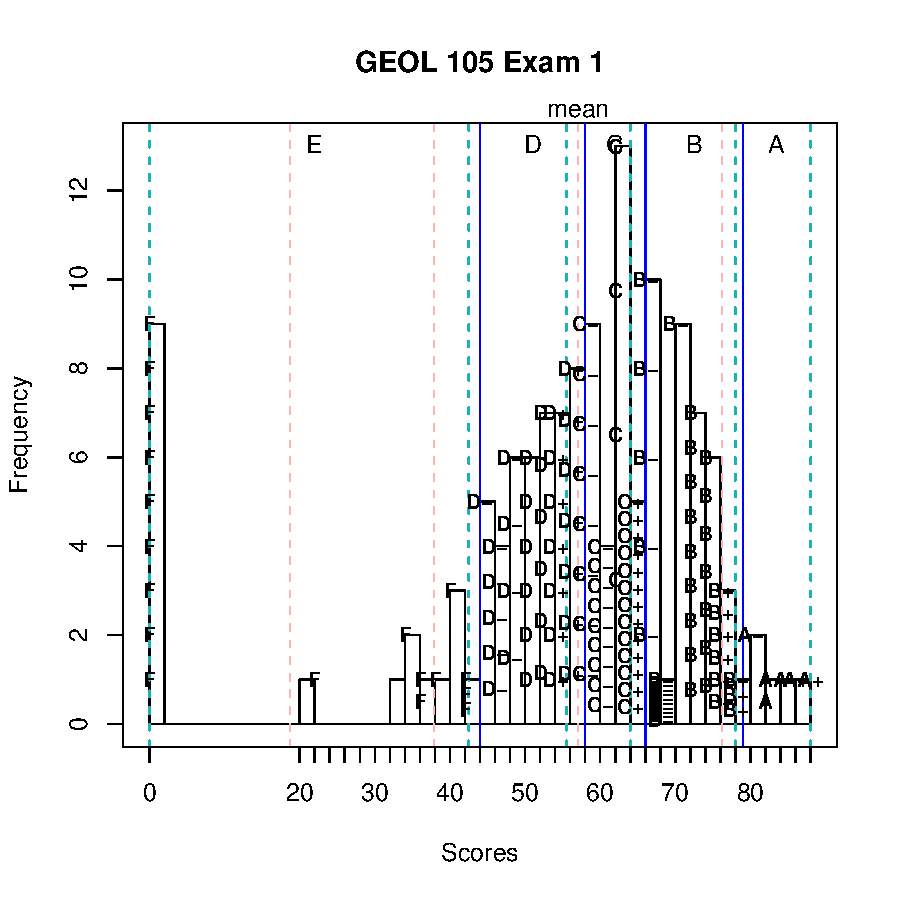
\includegraphics{grades-004}

showing all the letters grades plotted on the 
histogram.  Students can see their grade and
are often satisfied that they understand the 
idea of scaling.


\end{document}



